
\documentclass[a4paper,12pt]{article}

\usepackage{JYM-harj}
\usepackage{tikz}
\usepackage{amsmath}

\setlength{\parindent}{0in}

\setlength{\voffset}{-1.0cm}
\addtolength{\textheight}{2.0cm}

\setlength{\hoffset}{-1.0cm}
\addtolength{\textwidth}{2.0cm}

\usepackage{graphicx}
\usepackage{verbatim}

\usepackage{hyperref}

%\usepackage[finnish]{babel}
%\usepackage[utf8]{inputenc}
%\usepackage[T1]{fontenc}
%\usepackage{amsmath,amsfonts,amssymb,amsthm,amscd}


% 1: Teht\"av\"at
% 2: Kaikki ratkaisut
% 3: T\"ahdett\"om\"at ratkaisut
% 4: T\"ahdelliset ratkaisut
\newcommand{\tversio}{1}

\newcommand{\harjoitusnro}{3.3.2026 klo 17:00}

\ifthenelse{\tversio = 1}{\pagestyle{empty}}{}

\begin{document} 

\otsikko

\begin{enumerate}

\item 
    \begin{enumerate}
    \end{enumerate}
    
\item 
\begin{enumerate}
    \item Oheinen kuvio esittää funktiota $f : [0,5] \to [0,7]$. Vastaa seuraaviin kysymyksiin kuvan pohjalta: Onko funktio $f$ injektio? Onko se surjektio? Onko se bijektio? (Musta ja valkoinen ympyrä tarkoittavat sitä, että funktion arvoksi kohdassa $x=1$ on asetettu
$f(1)=0$, eli mustan ympyrän antama arvo.) \\
\\
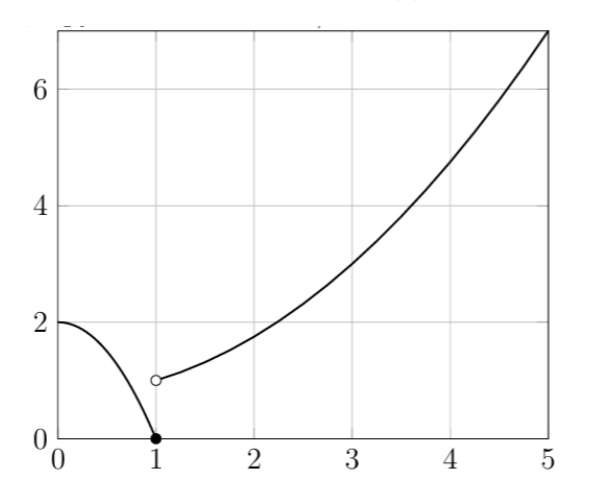
\includegraphics[width=0.5\textwidth]{brave_xz2GdHcPeq.png} \\
    \item Tarkastellaan relaatiota $R$, joka on määritelty reaalilukujen joukossa ehdolla
\[
xRy \quad \text{jos ja vain jos} \quad 2 \ge x-y \ge 1.
\]
Perustele esimerkein, miksi relaatio ei ole refleksiivinen,
symmetrinen eikä transitiivinen. \\
\end{enumerate}

\textbf{Vastaus:}

\begin{enumerate}
    \item \textbf{Onko f injektio?} Ei ole. Jos vedettäisiin vaakasuora viiva esim. kohtaan $y=1.5$, se leikkaisi funktion kuvaajan kahdessa eri pisteessä, kerran ennen ykköstä x-akselilla ja toisen kerran ykkösen oikealla puolella x-akselilla. 
    
    \textbf{Onko f surjektio?} Kyllä. Kuvaaja nousee seitsemään asti. Kaikki maalijoukon arvot välillä $[0,7]$ saavutetaan jollain x:n arvolla. Vasen osa kuvaajasta kattaa maalijoukon arvot kahdesta nollaan, ja oikea osa kuvaajasta yhdestä seitsemään. 

    \textbf{Onko f bijektio?} Ei ole. Jotta f olisi bijektio, sen täytyisi olla sekä injektio, että surjektio. Kuten edellä todistimme, f on kyllä surjektio, mutta ei injektio. Täten f ei ole bijektio. 

    \item Relaation $xRy$ voi ilmaista myös niin, että $x$ on relaatiossa muuttujan $y$ kanssa jos ja vain jos niiden erotus on välillä $[1,2]$. Seuraavaksi perustellaan vastaesimerkeillä miksi relaatio ei ole refleksiivinen, symmetrinen eikä transitiivinen.

    \textbf{Miksi R ei ole refleksiivinen?} Jotta R olisi refleksiivinen, täytyisi epäyhtälön $\quad 2 \ge x-x \ge 1$ olla tosi. Kaikilla  reaaliluvuilla $x-x=0$. Esim. jos $x=1$, saadaan $1-1=0$. Erotuksen tulos ei ole välillä $[1,2]$ eikä $1R1$ päde. Täten R ei ole refleksiivinen.

    \textbf{Miksi R ei ole symmetrinen?} Jotta $R$ olisi symmetrinen, täytyisi päteä sekä $xRy$, että $yRx$. Esim. jos valitaan $x=2$ ja $y=1$, ja asetetaan $x-y=2-1=1$ niin tämä kyllä toimii, mutta toisin päin $y-x=1-2=-1$ relaatio R ei päde koska $-1$ ei ole välillä $[1,2]$. Relaatio ei siis ole symmetrinen.

    \textbf{Miksi R ei ole transitiivinen?} Jotta R olisi transitiivinen, täytyisi siitä, että $xRy$ ja $yRz$ pätee, seurata se, että myös $xRz$ pätee. Esim. jos valitaan luvut $x=4$, $y=2.5$ ja $z=1$, saadaan tilanne, jossa transitiivisyys ei toteudu. $xRy$ toimii: $4-2.5=1.5$; tulos on välillä $[1,2]$ joten $4R2.5$ on tosi. $yRz$ toimii: $2.5-1=1.5$; tulos on välillä $[1,2]$ joten $2.5R1$ on tosi. Mutta $xRz$ ei toimi: $4-1=3$; tulos ei ole välillä $[1,2]$ joten $4R1$ on epätosi. Relaatio R ei täten ole transitiivinen. 

\end{enumerate}

\end{enumerate}

\end{document}